Nástrojů jak dnes psát dokumenty máme celou řadu, některé jsou volně dostupné a jiné jsou zpoplatněny. Některé nástroje jsme si již představili (Word, LibreOffice), ale
nyní se zaměříme na takzvané značkovací jazyky. Značkovací jazyky nám umožnují psát text, který je poté možné zpracovat počítačem, který změní jeho formátování. Většina
značkovacích jazyků má jasně\linebreak rozlišitelné značky, nebo jinak také tagy, které upravují formátování při jejich strojovém překladu, díky tomu je původní text stále dobře čitelný.
\cite{markup}

Mezi značkovací jazyky například patří i jazyky používané při\linebreak psaní webových stránek, jako je \gls{html} či \gls{xml}, ovšem tyto jazyky budeme spíše využívat pro zobrazování výstupu
jednodušších značkovacích jazyků jako je například \mbox{Markdown}.

\clearpage

\section{Markdown}

Markdown je značkovací jazyk, který převádí text do \gls{html}. Jedná se o jednoduše čitelný a zároveň jednoduchý jazyk na psaní strukturovaného textu. Hlavní myšlenkou Markdown je, že
text v něm psaný by měl být publikovatelný i bez jeho zpracování, inspirací tomuto přístupu jsou čistě textové emaily (emaily se dnes ve většině případů píšou v \gls{html}
z důvodu grafického obsahu). \cite{markdown}

Markdown se používá v na některých verzovacích službách jako je například Github, ovšem v tomto případě se jedná o upravenou implementaci Markdown, která je rozšířena o další
tagy/značky. Podobnou úpravu Markdown má i konkurenční služba GitLab.

Takto vypadá menší ukázka Markdown syntaxe a také výsledek, který je poté generován \ref{fig:markdown}.

\inputminted[linenos,breaklines]{md}{example.md}

\clearpage

\section{reStructuredText}

Formát reStructuredText pro psaní dokumentů v prostém textu, který je jednoduchý na čtení, kde je hned zřejmé jak bude vygenerovaný text vypadat.
Tento formát je jednoduchý na použití hlavně pro psaní programátorské dokumentace, jednoduchých webů a samostatných dokumentů.
Hlavním cílem reStructuredText je definovat a uplatnit jednoduchý značkovací jazyk pro použítí v Python, kde se používá k dokumentaci jednotlivých částí programu,
a dalších dokumentačních nástrojích, který je jednoduše čitelný a jednoduše použitelný. \cite{reStruDoc}

\uv{Docutil je open-source program pro zpracovaní dokumentace v textové podobě do, pro uživatele, přívětivého formátu, jako je například \gls{html}, \LaTeX~či \gls{xml}.} \cite{docutil}
Docutil používá jako vstupní formát již zmíněný reStructuredText. Pro převod do formátu \gls{pdf} lze poté použít utilitu Pandoc, která umí převěst různé značkovací jazyky
na ostatní formáty jako například náš rst (reStructuredText formát) a to nejenom do \gls{pdf}, ale také do formátů jako je Markdown, \gls{html} a dalších.
Pandoc lze také přímo využít v pythonu, díky modulu \textit{pypandoc}.

Stejně jako u Markdown, zde máme ukázku syntaxe i výsledného dokumentu. \ref{fig:rstOutput}

\inputminted[linenos,breaklines]{rst}{example-rst.rst}
\inputminted[linenos,breaklines]{rst}{module.rst}

\clearpage

\section{AsciiDoc}

AsciiDoc je další formát pro psaní dokumentu, jedná se stejně jako reStructuredText, o modul pro jazyk python. Tento modul je možné použít pro psaní nejenom poznámek,
ale je možné jej exportovat i do formátů jako jsou .epub (formát pro elektronické čtečky knih), či \gls{pdf}. \cite{asciiDoc} Syntaxe jazyku je podobná reStructuredText.

Projekt byl původně psán pro jazyk python, ovšem posléze byla syntaxe adoptována jako balíček pro jazyk ruby a také přejmenován na AsciiDoctor. AsciiDoctor lze posléze
použít i přímo v kódu, a to konkrétně v jazyce ruby, zde je menší ukázka nejenom formátu asciiDoc, ale i jeho použití v kódu.

Ani u AsciiDoc nesmíme zapomentou na ukázku syntaxe a výsledného dokumentu. \ref{fig:asciiOutput}

\inputminted[linenos,breaklines]{text}{example-ascii.adoc}
\inputminted[linenos,breaklines]{text}{module.adoc}
\begin{minted}[linenos,breaklines]{ruby}
    # example.rb
    require 'asciidoctor'

    Asciidoctor.convert_file 'example.adoc', to_file: true, safe: :safe
\end{minted}

\clearpage

\section{Porovnání}

Mezi jednotlivými jazyky nejsou velké rozdíly, ovšem v rámci řešení problému modularity textu má Markdown tu nevýhodu, že nelze vytvořit jednoduše modulární dokument.
Jazyk jako takový to nepodporuje a naše aplikace, by tedy musela umět text předzpracovat, než bychom mohli použít standardní překlad. To AsciiDoc i reStructuredText
mají oba možnost libovolného vkládání rozšiřujících souborů/modulů, tudíž není nutné text nijak předzpracovávat, pouze stačí dodržet správné cesty k souborům, které
chceme vkládat. Vše je tedy o rozhodnutí, který jazyk budeme chtít použít (ruby nebo python), neboť AsciiDoc pro python je již neudržovaný (není ani podpořena
verze 3 jazyka python).

\begin{figure}[h]
    \centering
    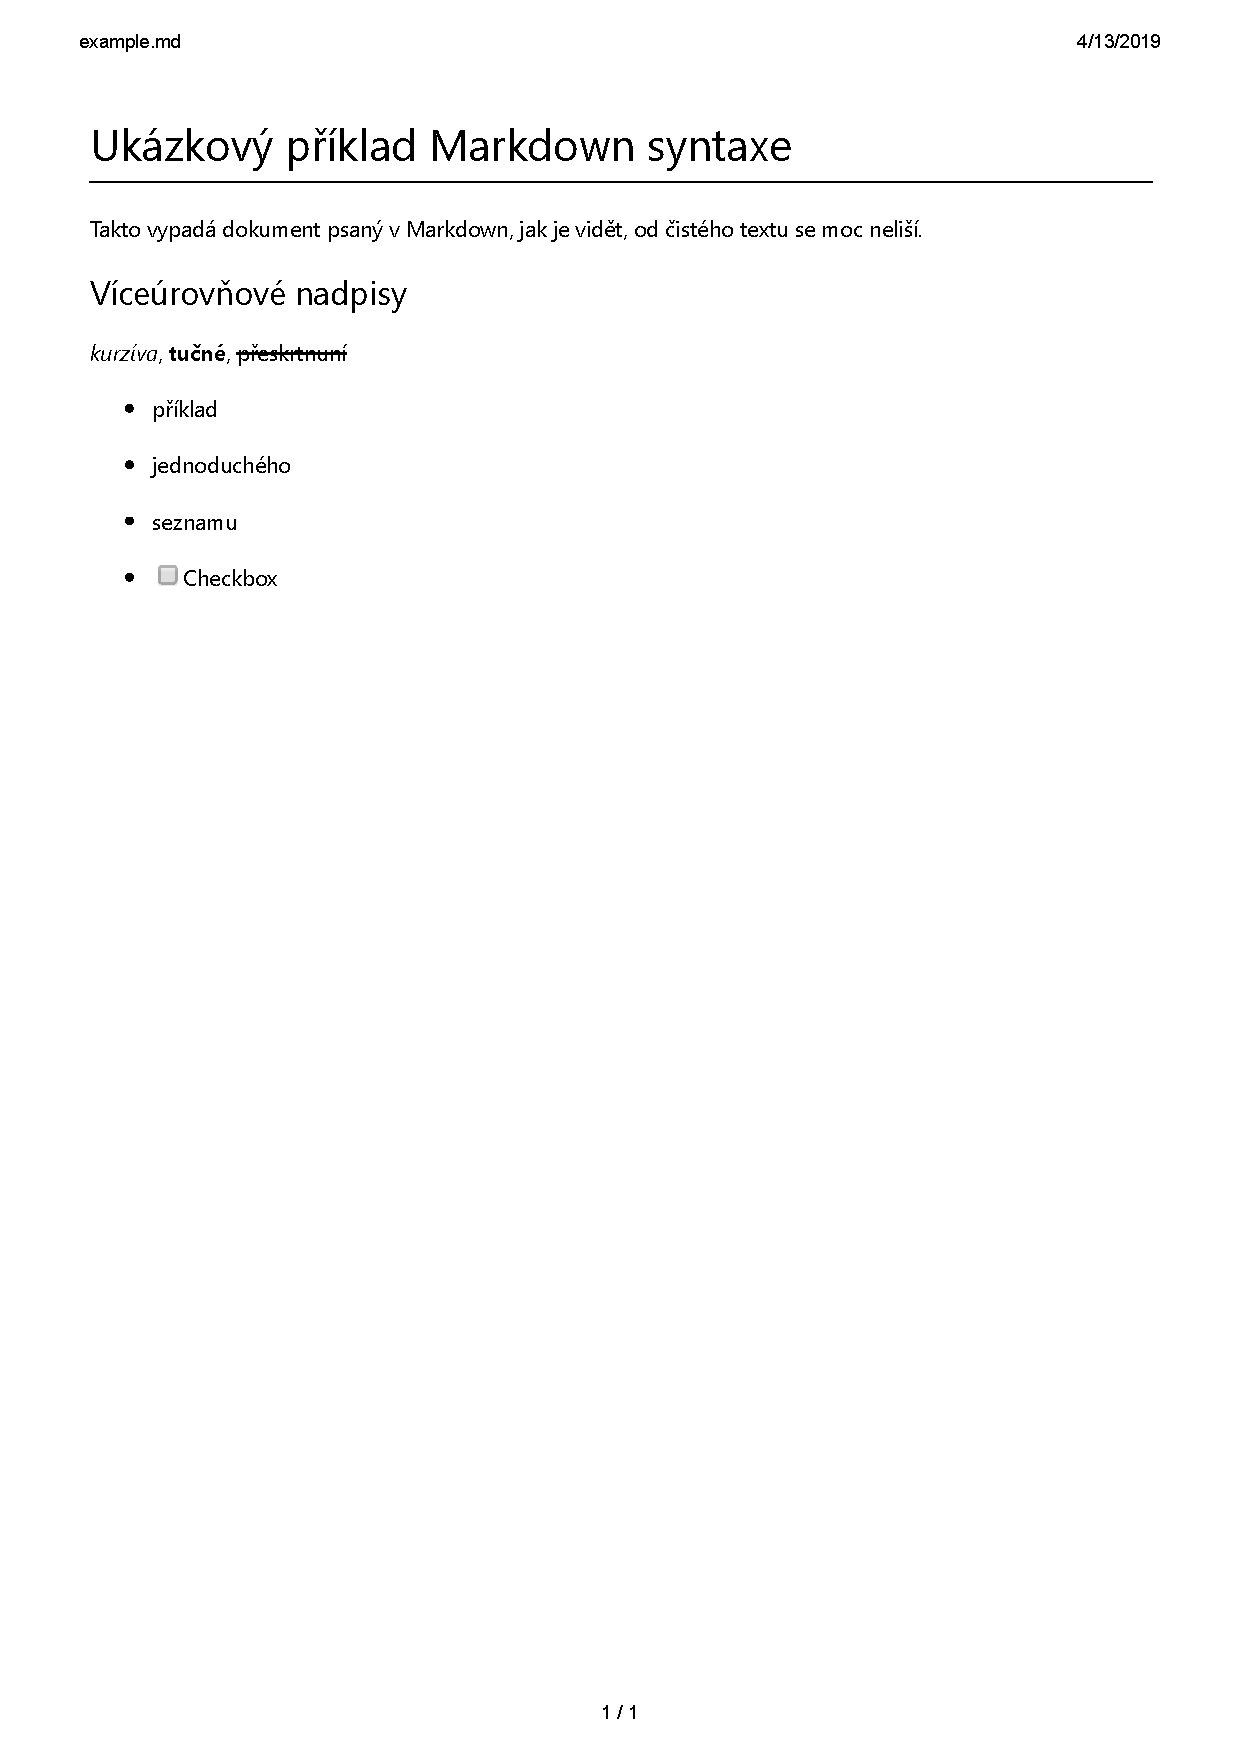
\includegraphics[width=\textwidth]{example.pdf}
    \caption{Výstup Markdown}
    \label{fig:markdown}
\end{figure}

\begin{figure}[h]
    \centering
    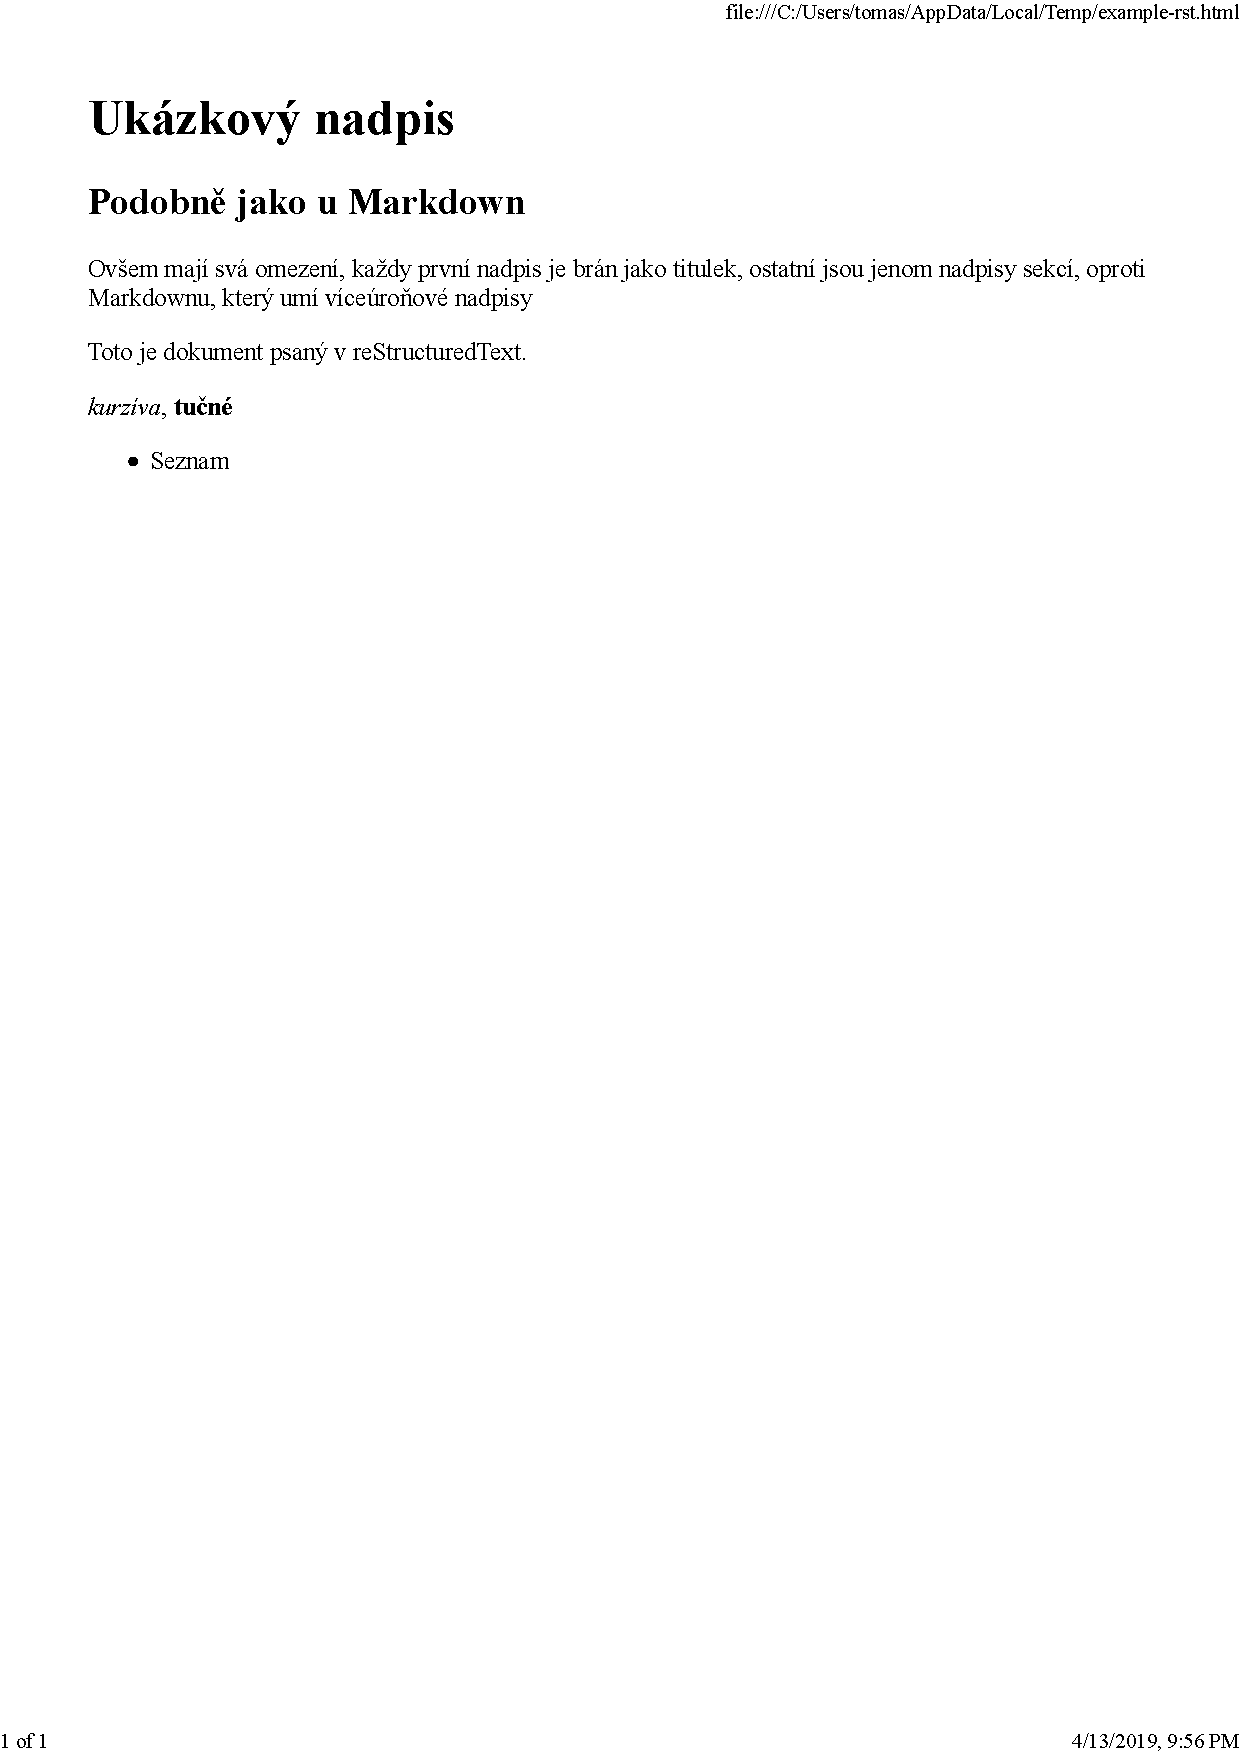
\includegraphics[width=\textwidth]{example-rst.pdf}
    \caption{Výstup reStructuredText}
    \label{fig:rstOutput}
\end{figure}

\begin{figure}[h]
    \centering
    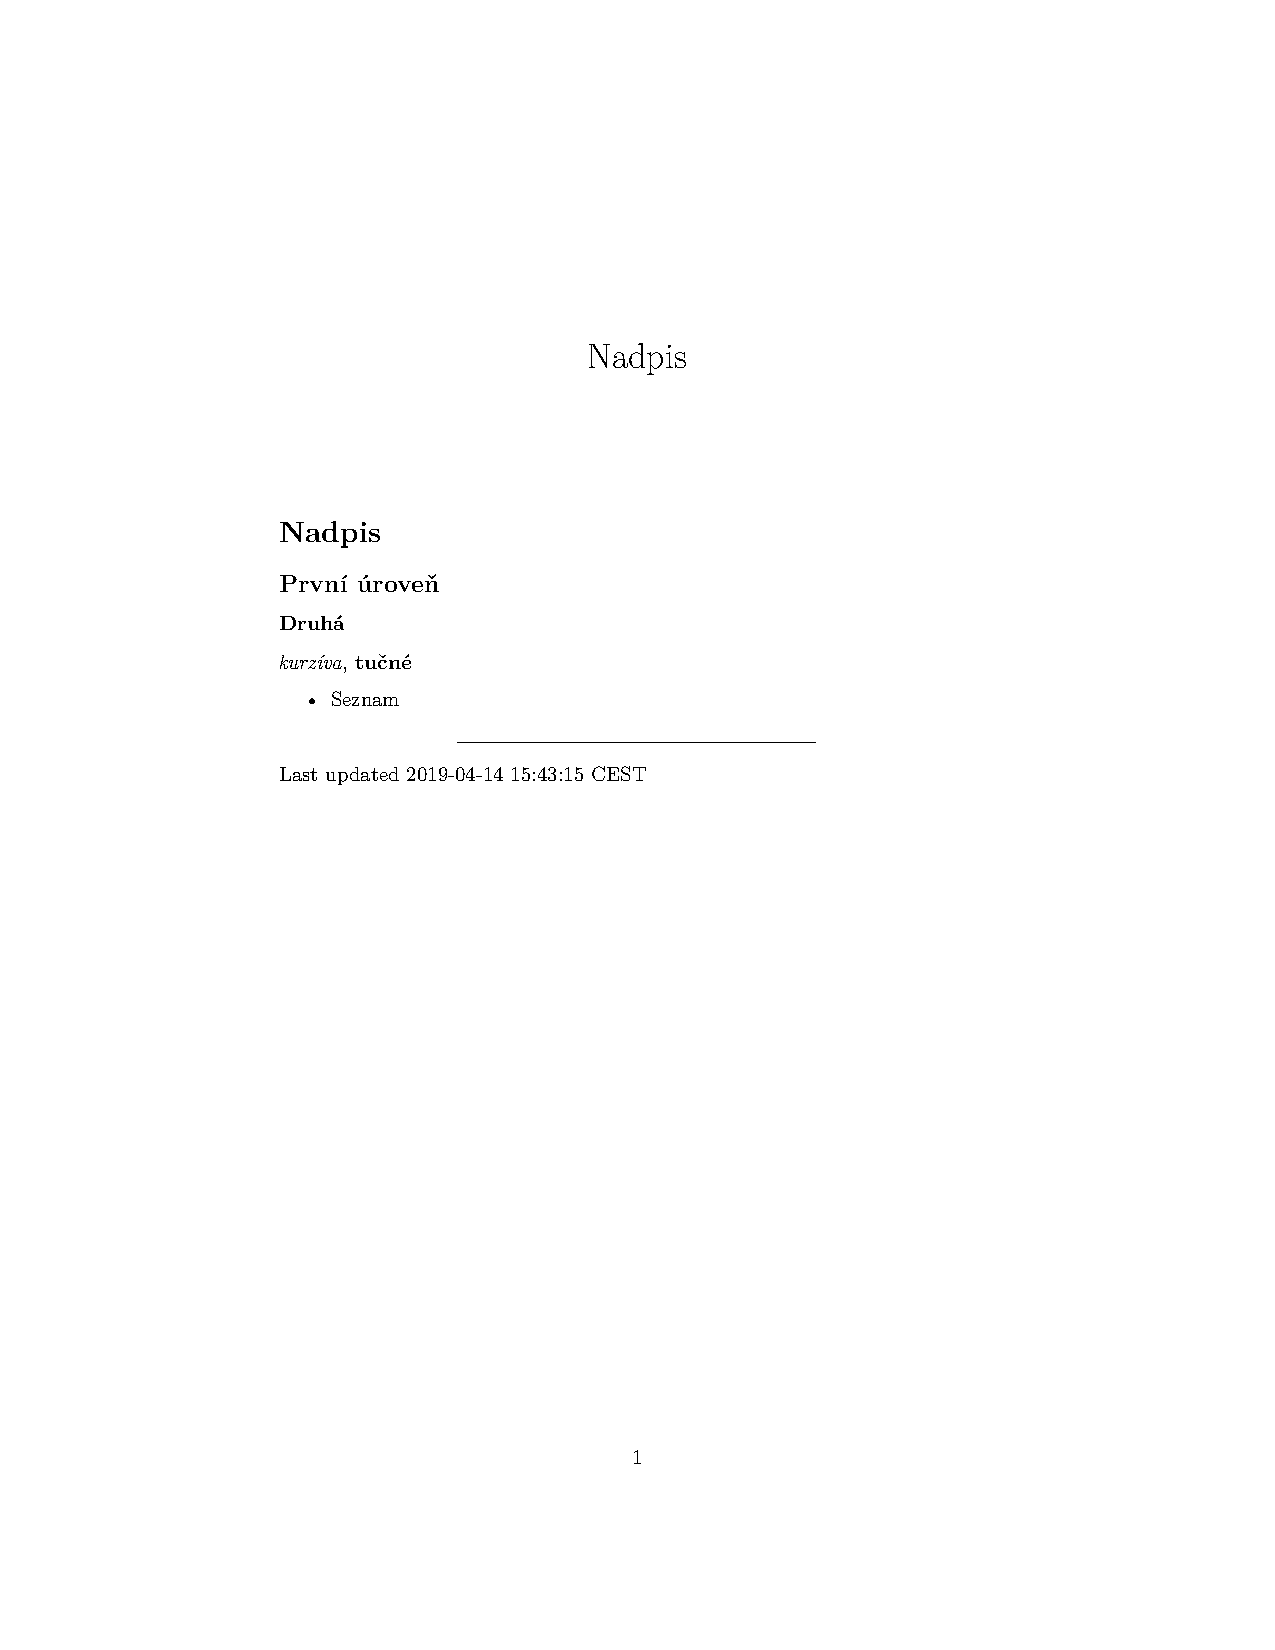
\includegraphics[width=\textwidth]{example-ascii.pdf}
    \caption{Výstup AsciiDoc}
    \label{fig:asciiOutput}
\end{figure}
